
%
% File sem_syn_diff.tex

\documentclass[11pt,a4paper]{article}
\usepackage[hyperref]{acl2018}
\usepackage{times}
\usepackage{latexsym}
\usepackage{amsmath}
\usepackage{tikz}
\usepackage{tikz-dependency}
\usepackage[warn]{textcomp}
\usepackage[font=small]{caption}
\usepackage{subcaption}
\usepackage{multirow}
\usepackage{url}
\usepackage{etoolbox}
\usepackage{xr}
\externaldocument{acl2018_supp}

\newcommand{\com}[1]{}
\newcommand{\oa}[1]{\footnote{\color{red}OA: #1}}
\newcommand{\daniel}[1]{\footnote{\color{blue}Daniel: #1}}

\hyphenation{SemEval}

\DeclareMathOperator*{\argmin}{argmin}
\DeclareMathOperator*{\argmax}{argmax}

\makeatletter
\patchcmd\@combinedblfloats{\box\@outputbox}{\unvbox\@outputbox}{}{%
   \errmessage{\noexpand\@combinedblfloats could not be patched}%
}%
 \makeatother


\usetikzlibrary{shapes,shapes.misc}

%\aclfinalcopy % Uncomment this line for the final submission
\def\aclpaperid{600}

%\setlength\titlebox{5cm}
% You can expand the titlebox if you need extra space
% to show all the authors. Please do not make the titlebox
% smaller than 5cm (the original size); we will check this
% in the camera-ready version and ask you to change it back.

\title{Is Semantic Representation Just Fancy Syntax?}

\author{Daniel Hershcovich$^{1,2}$ \\
  \\\And
  Omri Abend$^2$ \\
  $^1$The Edmond and Lily Safra Center for Brain Sciences \\
  $^2$School of Computer Science and Engineering \\
  Hebrew University of Jerusalem \\
  \texttt{\{danielh,oabend,arir\}@cs.huji.ac.il}
  \\\And
  Ari Rappoport$^2$
}

\date{}

\begin{document}

\maketitle

\begin{abstract}
\end{abstract}

\section{Introduction}\label{sec:introduction}

Semantic representation schemes have seen major progress in recent years.
In parallel, syntactic representation is becoming more semantic.
However, looking at the absolute scores achieved in semantic parsing tasks
as opposed to syntactic parsing,
there is still a gap:
UCCA parsers get just about 75\% F-score, whereas UD parsers get more than 85\% LAS F1. Why?
UD has much more training data (UCCA: 5K, UD: about17K for English).
But inter-annotator agreement is also lower: about 85\% for UCCA, and more than 95\% for UD.

Several questions naturally manifest themselves:
how much of the difference is explained by the differences in---
\begin{itemize}
\item Evaluation metric,
\item Amount of training data,
\item Content.
\end{itemize}

The gap can be explained by adposition and case supersenses
\cite{schneider2017adposition,blodgett2018semantic}.

%%%%%%%%%%%%%%%%%%%%%%%%%%%%%%%%%%%%%%%%%%%%%%%%%%%%%%%%%%%%%%%%%%%%%%%%%%%%%%%%%
\section{Related Work}\label{sec:related_work}

\begin{figure}[!ht]
\fbox{\begin{subfigure}{0.47\textwidth}
  \centering
  \scalebox{.95}{
  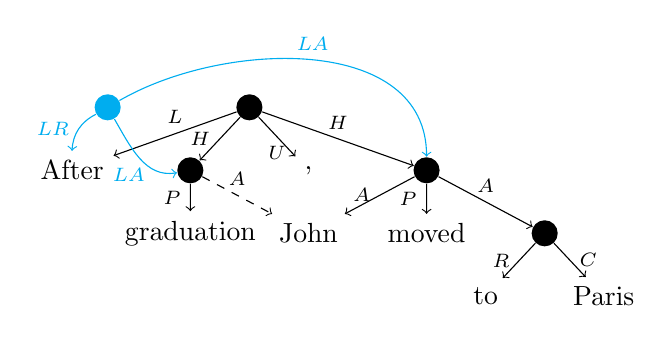
\begin{tikzpicture}[level distance=8mm, ->]
    \node (ROOT) [fill=black, circle] {}
      child {node (After) {After} edge from parent node[above] {\scriptsize $L$}}
      child {node (graduation) [fill=black, circle] {}
      {
        child {node {graduation} edge from parent node[left] {\scriptsize $P$}}
      } edge from parent node[left] {\scriptsize $H$} }
      child {node {,} edge from parent node[below] {\scriptsize $U$}}
      child {node (moved) [fill=black, circle] {}
      {
        child {node (John) {John} edge from parent node[left] {\scriptsize $A$}}
        child {node {moved} edge from parent node[left] {\scriptsize $P$}}
        child {node [fill=black, circle] {}
        {
          child {node {to} edge from parent node[left] {\scriptsize $R$}}
          child {node {Paris} edge from parent node[right] {\scriptsize $C$}}
        } edge from parent node[above] {\scriptsize $A$} }
      } edge from parent node[above] {\scriptsize $H$} }
      ;
    \draw[dashed,->] (graduation) to node [above] {\scriptsize $A$} (John);
    \node (LKG) at (-1.8,0) [fill=cyan, circle] {};
    \draw[bend right,color=cyan] (LKG) to node [auto, left] {\scriptsize $LR$} (After);
    \draw[color=cyan] (LKG) to[out=-60, in=190] node [below] {\scriptsize $LA\quad$} (graduation);
    \draw[color=cyan] (LKG) to[out=30, in=90] node [above] {\scriptsize $LA$} (moved);
  \end{tikzpicture}
  }\caption{UCCA \label{fig:original_example_ucca}}
\end{subfigure}}

\caption{\label{fig:original_examples}}

\citet{wang2015transition,wang-xue-pradhan:2015:ACL-IJCNLP,wang-EtAl:2016:SemEval,goodman2016noise,wang2017getting}
presented a transition-based AMR parser, CAMR, which requires a
syntactic dependency tree as input.
It operates on the input tree, transforming it into an AMR graph
by a sequence of transitions.
The accuracy of the underlying syntactic dependency parser is important,
as shown by \citet{wang-xue-pradhan:2015:ACL-IJCNLP},
who achieved the best results using the Charniak parser trained on a
much larger and more diverse dataset---the full OntoNotes corpus,
rather than the Stanford parser trained on the Penn TreeBank.

\end{figure}


%%%%%%%%%%%%%%%%%%%%%%%%%%%%%%%%%%%%%%%%%%%%%%%%%%%%%%%%%%%%%%%%%%%%%%%%%%%%%%%%%

\paragraph{Universal Conceptual Cognitive Annotation.}\label{sec:ucca}
UCCA \cite{abend2013universal} is a semantic representation whose main design principles
are ease of annotation, cross-linguistic applicability, and a modular architecture.
%of semantic distinctions.
UCCA represents the semantics of linguistic utterances
as directed acyclic graphs (DAGs), where terminal (childless) nodes
correspond to the text tokens, and non-terminal nodes to semantic units that participate
in some super-ordinate relation.
Edges are labeled, indicating the role of a child in the relation the parent represents.
Nodes and edges belong to one of several \textit{layers}, each corresponding
to a ``module'' of semantic distinctions.
UCCA's \textit{foundational layer} (the only layer for which annotated data exists)
mostly covers predicate-argument structure, semantic heads and inter-Scene relations.
%The \textit{linkage} layer covers relations between events, including temporal and discourse relations
%(exemplified by the gray node and its outgoing edges in Figure~\ref{fig:original_example_ucca}).

UCCA distinguishes \textit{primary} edges, corresponding 
to explicit relations, from \textit{remote} edges (appear dashed in
Figure~\ref{fig:original_example_ucca}) that allow for a unit to participate
in several super-ordinate relations.
Primary edges form a tree in each layer, whereas remote edges enable reentrancy, forming a DAG.
%As UCCA annotated data is currently fairly scarce (see \S\ref{sec:experiments}), 
%we hypothesize it will benefit from MTL, and consider it as our
%main task.


\section{Amount of training data}

Syntactic dependency parsers require many training examples to achieve
state-of-the-art results.
Even after around 500K tokens, the learning curves do not seem to saturate
\cite{de2017old,velldal2017joint}.



\section{Experiments}\label{sec:experiments}

\begin{table*}[t]
\centering
\small
\setlength\tabcolsep{2pt}
\begin{tabular}{l|ccc|ccc||ccc|ccc||ccc|ccc}
& \multicolumn{6}{c||}{\footnotesize \bf English}
& \multicolumn{6}{c||}{\footnotesize \bf French}
& \multicolumn{6}{c}{\footnotesize \bf German} \\
\hline
& \multicolumn{3}{c|}{\footnotesize \bf {\#} tokens}
& \multicolumn{3}{c||}{\footnotesize \bf {\#} sentences}
& \multicolumn{3}{c|}{\footnotesize \bf {\#} tokens}
& \multicolumn{3}{c||}{\footnotesize \bf {\#} sentences}
& \multicolumn{3}{c|}{\footnotesize \bf {\#} tokens}
& \multicolumn{3}{c}{\footnotesize \bf {\#} sentences} \\
& \footnotesize \bf train & \footnotesize \bf dev & \footnotesize \bf test
& \footnotesize \bf train & \footnotesize \bf dev & \footnotesize \bf test
& \footnotesize \bf train & \footnotesize \bf dev & \footnotesize \bf test 
& \footnotesize \bf train & \footnotesize \bf dev & \footnotesize \bf test
& \footnotesize \bf train & \footnotesize \bf dev & \footnotesize \bf test
& \footnotesize \bf train & \footnotesize \bf dev & \footnotesize \bf test \\
\hline
Wiki & 128444 & 14676 & 15313 & 4268 & 454 & 503 &&&&&&&&&&&& \\
20K &&& 12339 &&& 506 & 10047 & 1558 & 1324 & 413 & 67 & 67 & 79894 & 10059 & 42366 & 3429 & 561 & 2164
\end{tabular}
\caption{Number of tokens and sentences in the training, development and test sets
we use for each corpus and language.\label{tab:corpora}}
\end{table*}

\paragraph{Data.}

For UCCA, we use v1.2 of the English Wikipedia corpus \cite[\textit{Wiki};][]{abend2013universal},
with the standard train/dev/test split (see Table~\ref{tab:corpora}),
and the \textit{Twenty Thousand Leagues Under the Sea} corpora
\cite[\textit{20K};][]{sulem2015conceptual},
annotated in English, French and German.\footnote{\mbox{\url{http://github.com/huji-nlp/ucca-corpora}}}
For English and French we use 20K v1.0,
a small parallel corpus comprising the first five chapters of the book.
As in previous work \cite{hershcovich2017a}, we use the English part only as an out-of-domain test set.
We train and test on the French part using the standard split,
as well as the German corpus (v0.9),
which is a pre-release and still contains a considerable amount of noisy annotation.
Tuning is performed on the respective development sets.

\paragraph{Experimental setup.}


\paragraph{Evaluation.}



\section{Results}\label{sec:results}

\section{Discussion}\label{sec:discussion}


\section{Conclusion}\label{sec:conclusion}


\bibliography{references}
\bibliographystyle{acl_natbib}

\end{document}
